\section{Validation on Synthetic Benchmark}
\label{sec:synthetic}

To examine the measures where the answer is known before evaluating large-scale models, we implemented a controlled synthetic toy-fusion benchmark with known data-generating distributions. The benchmark evaluates three distinct architectural designs:
\begin{enumerate}
    \item \textbf{FixedModel}: A quality-blind linear fusion baseline with constant equal weighting across modalities.
    \item \textbf{PartialGatedModel}: A heuristic gating model that partially dampens degraded inputs.
    \item \textbf{GatedModel}: A quality-aware gated architecture that dynamically dampens inputs as noise increases.
\end{enumerate}

\subsection{Empirical Validation Results}
Table~\ref{tab:synthetic-summary} reports the empirical crossing points $S^*$ and Misalignment Index ($\mi$) across five independent random seeds under the removed null baseline.

\begin{figure}[tb]
\centering
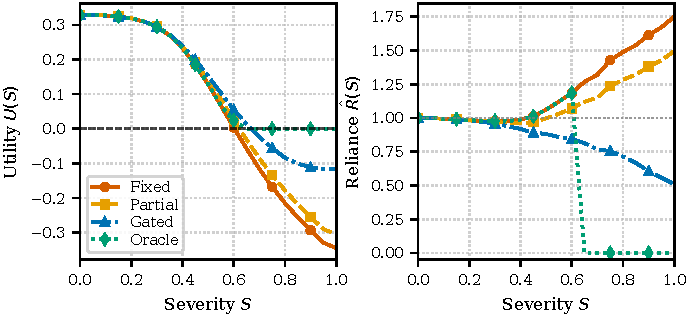
\includegraphics[width=\textwidth]{figures/fig1_synthetic_two_panel.pdf}
\caption{Synthetic benchmark ($N=2000$ test items per seed, 5 seeds, removed null baseline, bootstrap $B=1000$, seed 42). Left: utility $U(S)$ versus severity for Fixed, Partial, Gated, and Oracle models. Right: normalized reliance $\hat R(S)$. The quality-aware Gated model achieves the lowest misalignment.}
\label{fig:synthetic}
\end{figure}

\begin{table}[t]
\centering
\caption{Synthetic benchmark results across architectures and null baselines (Iteration v0.4, $N=2000$ test items per seed, 5 seeds, bootstrap $B=1000$, seed 42).}
\label{tab:synthetic-summary}
\fittable{%
\begin{tabular}{llccccc}
\toprule
\textbf{Model} & \textbf{Null} & \textbf{Clean Acc} & \textbf{Null Acc} & $S^*$ & $\text{MI}_{\text{pooled}}$ & $\text{MI}_{\text{hier}}$ \\
\midrule
Fixed & removed & 0.996 & 0.667 & 0.650 (0.600, 0.650) & 1.491 (1.454, 1.507) & 1.491 (1.373, 1.637) \\
Fixed & zeros & 0.996 & 0.413 & 0.850 (0.850, 0.900) & 0.726 (0.717, 0.741) & 0.726 (0.581, 0.877) \\
Fixed & mean & 0.996 & 0.367 & 0.950 (0.900, 0.950) & 0.862 (0.847, 0.876) & 0.862 (0.670, 1.012) \\
Partial Gated & removed & 0.996 & 0.667 & 0.650 (0.650, 0.650) & 1.286 (1.267, 1.305) & 1.286 (1.196, 1.405) \\
Partial Gated & zeros & 0.996 & 0.416 & 0.900 (0.900, 0.950) & 0.638 (0.629, 0.651) & 0.638 (0.504, 0.781) \\
Partial Gated & mean & 0.996 & 0.377 & 0.950 (0.950, 0.950) & 0.774 (0.766, 0.792) & 0.774 (0.583, 0.927) \\
Gated & removed & 0.996 & 0.667 & 0.700 (0.700, 0.700) & 0.650 (0.639, 0.661) & 0.650 (0.579, 0.752) \\
Gated & zeros & 0.996 & 0.422 & no crossing & no crossing & no crossing \\
Gated & mean & 0.996 & 0.386 & no crossing & no crossing & no crossing \\
Oracle Gated & removed & 0.996 & 0.667 & 0.700 (0.650, 0.700) & 0.000 (0.000, 0.000) & 0.000 (0.000, 0.208) \\
Oracle Gated & zeros & 0.996 & 0.413 & no crossing & no crossing & no crossing \\
Oracle Gated & mean & 0.996 & 0.367 & no crossing & no crossing & no crossing \\
Sharp gate x0.5 & removed & 0.995 & 0.667 & 0.700 (0.650, 0.700) & 0.862 (0.847, 0.876) & 0.862 (0.782, 0.967) \\
Sharp gate x0.5 & zeros & 0.995 & 0.428 & no crossing & no crossing & no crossing \\
Sharp gate x0.5 & mean & 0.995 & 0.401 & no crossing & no crossing & no crossing \\
Sharp gate x1.0 & removed & 0.996 & 0.667 & 0.700 (0.700, 0.700) & 0.650 (0.639, 0.662) & 0.650 (0.580, 0.758) \\
Sharp gate x1.0 & zeros & 0.996 & 0.422 & no crossing & no crossing & no crossing \\
Sharp gate x1.0 & mean & 0.996 & 0.386 & no crossing & no crossing & no crossing \\
Sharp gate x2 & removed & 0.995 & 0.667 & 0.700 (0.700, 0.700) & 0.511 (0.502, 0.522) & 0.511 (0.429, 0.630) \\
Sharp gate x2 & zeros & 0.995 & 0.423 & no crossing & no crossing & no crossing \\
Sharp gate x2 & mean & 0.995 & 0.373 & no crossing & no crossing & no crossing \\
Sharp gate x4 & removed & 0.994 & 0.667 & 0.650 (0.650, 0.700) & 0.470 (0.436, 0.480) & 0.470 (0.360, 0.572) \\
Sharp gate x4 & zeros & 0.994 & 0.444 & no crossing & no crossing & no crossing \\
Sharp gate x4 & mean & 0.994 & 0.368 & no crossing & no crossing & no crossing \\
Sharp gate x8 & removed & 0.992 & 0.667 & 0.650 (0.650, 0.650) & 0.440 (0.430, 0.449) & 0.440 (0.331, 0.545) \\
Sharp gate x8 & zeros & 0.992 & 0.454 & no crossing & no crossing & no crossing \\
Sharp gate x8 & mean & 0.992 & 0.367 & no crossing & no crossing & no crossing \\
Sharp gate x16 & removed & 0.991 & 0.667 & 0.650 (0.650, 0.650) & 0.425 (0.417, 0.434) & 0.425 (0.321, 0.539) \\
Sharp gate x16 & zeros & 0.991 & 0.455 & no crossing & no crossing & no crossing \\
Sharp gate x16 & mean & 0.991 & 0.367 & no crossing & no crossing & no crossing \\
\bottomrule
\end{tabular}}
\end{table}


Under the canonical \emph{removed} null baseline:
\begin{itemize}
    \item The quality-blind \textbf{FixedModel} crosses zero utility at $S^* \approx 0.65$ but maintains heavy predictive reliance, resulting in high misalignment ($\mi \approx \checknum{1.491}{synthetic:FixedModel:MI}$, 95\% CI $[\checknum{1.454}{synthetic:FixedModel:MI_lo}, \checknum{1.507}{synthetic:FixedModel:MI_hi}]$).
    \item The \textbf{PartialGatedModel} yields moderate misalignment ($\mi \approx \checknum{1.286}{synthetic:PartialGatedModel:MI}$, 95\% CI $[\checknum{1.267}{synthetic:PartialGatedModel:MI_lo}, \checknum{1.305}{synthetic:PartialGatedModel:MI_hi}]$).
    \item The quality-aware \textbf{GatedModel} exhibits substantially lower misalignment ($\mi \approx \checknum{0.650}{synthetic:GatedModel:MI}$, 95\% CI $[\checknum{0.639}{synthetic:GatedModel:MI_lo}, \checknum{0.661}{synthetic:GatedModel:MI_hi}]$).
\end{itemize}
The pre-declared comparison of independent hierarchical intervals for \textbf{FixedModel} and \textbf{PartialGatedModel} overlapped narrowly ($[1.373, 1.637]$ vs.\ $[1.196, 1.405]$), and the \textbf{GatedModel} misalignment of $\mi \approx \checknum{0.650}{synthetic:GatedModel:MI}$ did not reach the original 0.2 threshold. The paired bootstrap analysis show that the measures order the architectures as intended, although the first success criterion (Gated MI below 0.2) was not met.
